
\documentclass[tikz,convert={convertexe={magick.exe}}]{standalone}

\begin{document}
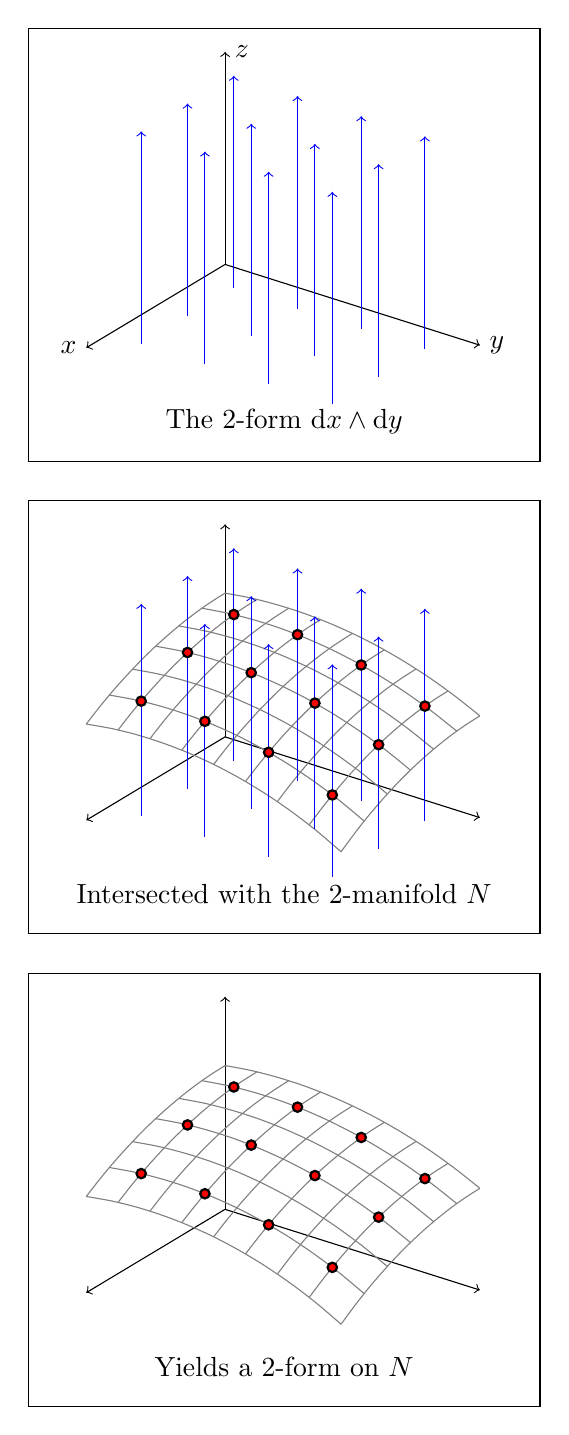
\begin{tikzpicture}

\tikzstyle atom=[circle, draw, inner sep=1.2pt, fill=red, thick]

\begin{scope}

\draw[->] (0.000,0.000)--(-1.763,-1.058) node[left]{$x$};
\draw[->] (0.000,0.000)--(3.236,-1.025) node[right]{$y$};
\draw[->] (0.000,0.000)--(0.000,2.700) node[right]{$z$};

\draw[->,blue] (0.111,-0.304)--(0.111,2.396);
\draw[->,blue] (0.920,-0.561)--(0.920,2.139);
\draw[->,blue] (1.729,-0.817)--(1.729,1.883);
\draw[->,blue] (2.538,-1.073)--(2.538,1.627);
\draw[->,blue] (-0.477,-0.657)--(-0.477,2.043);
\draw[->,blue] (0.332,-0.913)--(0.332,1.787);
\draw[->,blue] (1.141,-1.169)--(1.141,1.531);
\draw[->,blue] (1.950,-1.426)--(1.950,1.274);
\draw[->,blue] (-1.065,-1.010)--(-1.065,1.690);
\draw[->,blue] (-0.256,-1.266)--(-0.256,1.434);
\draw[->,blue] (0.553,-1.522)--(0.553,1.178);
\draw[->,blue] (1.362,-1.778)--(1.362,0.922);

\draw (-2.5,-2.5) rectangle (4,3);
\node at (0.75,-2) {The $2$-form $\mathrm{d}x \wedge \mathrm{d}y$};
\end{scope}

\begin{scope}[yshift = -6cm]
\draw[->] (0.000,0.000)--(-1.763,-1.058);
\draw[->] (0.000,0.000)--(3.236,-1.025);
\draw[->] (0.000,0.000)--(0.000,2.700);
\draw[gray] plot[smooth] coordinates{(0.000,1.826) (0.324,1.765) (0.647,1.682) (0.971,1.580) (1.294,1.457) (1.618,1.314) (1.942,1.150) (2.265,0.964) (2.589,0.756) (2.912,0.524) (3.236,0.267)};
\draw[gray] plot[smooth] coordinates{(-0.294,1.634) (0.030,1.572) (0.353,1.490) (0.677,1.388) (1.001,1.265) (1.324,1.122) (1.648,0.957) (1.971,0.771) (2.295,0.563) (2.619,0.330) (2.942,0.073)};
\draw[gray] plot[smooth] coordinates{(-0.588,1.409) (-0.264,1.348) (0.059,1.266) (0.383,1.164) (0.707,1.041) (1.030,0.897) (1.354,0.732) (1.677,0.545) (2.001,0.336) (2.325,0.103) (2.648,-0.156)};
\draw[gray] plot[smooth] coordinates{(-0.882,1.152) (-0.558,1.091) (-0.234,1.009) (0.089,0.907) (0.413,0.783) (0.736,0.639) (1.060,0.473) (1.384,0.286) (1.707,0.075) (2.031,-0.160) (2.354,-0.422)};
\draw[gray] plot[smooth] coordinates{(-1.176,0.860) (-0.852,0.800) (-0.528,0.718) (-0.205,0.616) (0.119,0.492) (0.442,0.347) (0.766,0.180) (1.090,-0.009) (1.413,-0.222) (1.737,-0.460) (2.060,-0.725)};
\draw[gray] plot[smooth] coordinates{(-1.469,0.531) (-1.146,0.472) (-0.822,0.391) (-0.499,0.289) (-0.175,0.165) (0.149,0.019) (0.472,-0.150) (0.796,-0.342) (1.119,-0.558) (1.443,-0.800) (1.767,-1.070)};
\draw[gray] plot[smooth] coordinates{(-1.763,0.163) (-1.440,0.106) (-1.116,0.026) (-0.793,-0.077) (-0.469,-0.202) (-0.145,-0.349) (0.178,-0.520) (0.502,-0.715) (0.825,-0.935) (1.149,-1.182) (1.473,-1.459)};
\draw[gray] plot[smooth] coordinates{(0.000,1.826) (-0.176,1.715) (-0.353,1.592) (-0.529,1.457) (-0.705,1.310) (-0.882,1.152) (-1.058,0.981) (-1.234,0.797) (-1.411,0.600) (-1.587,0.389) (-1.763,0.163)};
\draw[gray] plot[smooth] coordinates{(0.405,1.746) (0.228,1.635) (0.052,1.512) (-0.124,1.377) (-0.301,1.231) (-0.477,1.072) (-0.654,0.902) (-0.830,0.719) (-1.006,0.523) (-1.183,0.313) (-1.359,0.088)};
\draw[gray] plot[smooth] coordinates{(0.809,1.634) (0.633,1.522) (0.456,1.399) (0.280,1.265) (0.104,1.119) (-0.073,0.961) (-0.249,0.790) (-0.425,0.607) (-0.602,0.411) (-0.778,0.202) (-0.954,-0.023)};
\draw[gray] plot[smooth] coordinates{(1.214,1.490) (1.037,1.378) (0.861,1.255) (0.685,1.121) (0.508,0.974) (0.332,0.816) (0.156,0.646) (-0.021,0.463) (-0.197,0.266) (-0.373,0.056) (-0.550,-0.168)};
\draw[gray] plot[smooth] coordinates{(1.618,1.314) (1.442,1.202) (1.265,1.079) (1.089,0.944) (0.913,0.798) (0.736,0.639) (0.560,0.468) (0.384,0.284) (0.207,0.087) (0.031,-0.124) (-0.145,-0.349)};
\draw[gray] plot[smooth] coordinates{(2.023,1.105) (1.846,0.994) (1.670,0.870) (1.494,0.735) (1.317,0.588) (1.141,0.429) (0.965,0.257) (0.788,0.072) (0.612,-0.126) (0.436,-0.339) (0.259,-0.566)};
\draw[gray] plot[smooth] coordinates{(2.427,0.863) (2.251,0.751) (2.074,0.627) (1.898,0.491) (1.722,0.344) (1.545,0.183) (1.369,0.010) (1.193,-0.177) (1.016,-0.377) (0.840,-0.592) (0.664,-0.822)};
\draw[gray] plot[smooth] coordinates{(2.832,0.584) (2.655,0.472) (2.479,0.348) (2.303,0.212) (2.126,0.063) (1.950,-0.099) (1.774,-0.274) (1.597,-0.463) (1.421,-0.666) (1.245,-0.884) (1.068,-1.118)};
\draw[gray] plot[smooth] coordinates{(3.236,0.267) (3.060,0.155) (2.883,0.030) (2.707,-0.108) (2.531,-0.258) (2.354,-0.422) (2.178,-0.599) (2.002,-0.791) (1.825,-0.997) (1.649,-1.220) (1.473,-1.459)};
\draw[->,blue] (0.111,-0.304)--(0.111,2.396);
\node[atom] at (0.111,1.554) {};
\draw[->,blue] (0.920,-0.561)--(0.920,2.139);
\node[atom] at (0.920,1.298) {};
\draw[->,blue] (1.729,-0.817)--(1.729,1.883);
\node[atom] at (1.729,0.913) {};
\draw[->,blue] (2.538,-1.073)--(2.538,1.627);
\node[atom] at (2.538,0.391) {};
\draw[->,blue] (-0.477,-0.657)--(-0.477,2.043);
\node[atom] at (-0.477,1.072) {};
\draw[->,blue] (0.332,-0.913)--(0.332,1.787);
\node[atom] at (0.332,0.816) {};
\draw[->,blue] (1.141,-1.169)--(1.141,1.531);
\node[atom] at (1.141,0.429) {};
\draw[->,blue] (1.950,-1.426)--(1.950,1.274);
\node[atom] at (1.950,-0.099) {};
\draw[->,blue] (-1.065,-1.010)--(-1.065,1.690);
\node[atom] at (-1.065,0.454) {};
\draw[->,blue] (-0.256,-1.266)--(-0.256,1.434);
\node[atom] at (-0.256,0.198) {};
\draw[->,blue] (0.553,-1.522)--(0.553,1.178);
\node[atom] at (0.553,-0.196) {};
\draw[->,blue] (1.362,-1.778)--(1.362,0.922);
\node[atom] at (1.362,-0.737) {};

\draw (-2.5,-2.5) rectangle (4,3);
\node at (0.75,-2) {Intersected with the 2-manifold $N$};

\end{scope}

\begin{scope}[yshift=-12cm]
\draw[->] (0.000,0.000)--(-1.763,-1.058);
\draw[->] (0.000,0.000)--(3.236,-1.025);
\draw[->] (0.000,0.000)--(0.000,2.700);
\draw[gray] plot[smooth] coordinates{(0.000,1.826) (0.324,1.765) (0.647,1.682) (0.971,1.580) (1.294,1.457) (1.618,1.314) (1.942,1.150) (2.265,0.964) (2.589,0.756) (2.912,0.524) (3.236,0.267)};
\draw[gray] plot[smooth] coordinates{(-0.294,1.634) (0.030,1.572) (0.353,1.490) (0.677,1.388) (1.001,1.265) (1.324,1.122) (1.648,0.957) (1.971,0.771) (2.295,0.563) (2.619,0.330) (2.942,0.073)};
\draw[gray] plot[smooth] coordinates{(-0.588,1.409) (-0.264,1.348) (0.059,1.266) (0.383,1.164) (0.707,1.041) (1.030,0.897) (1.354,0.732) (1.677,0.545) (2.001,0.336) (2.325,0.103) (2.648,-0.156)};
\draw[gray] plot[smooth] coordinates{(-0.882,1.152) (-0.558,1.091) (-0.234,1.009) (0.089,0.907) (0.413,0.783) (0.736,0.639) (1.060,0.473) (1.384,0.286) (1.707,0.075) (2.031,-0.160) (2.354,-0.422)};
\draw[gray] plot[smooth] coordinates{(-1.176,0.860) (-0.852,0.800) (-0.528,0.718) (-0.205,0.616) (0.119,0.492) (0.442,0.347) (0.766,0.180) (1.090,-0.009) (1.413,-0.222) (1.737,-0.460) (2.060,-0.725)};
\draw[gray] plot[smooth] coordinates{(-1.469,0.531) (-1.146,0.472) (-0.822,0.391) (-0.499,0.289) (-0.175,0.165) (0.149,0.019) (0.472,-0.150) (0.796,-0.342) (1.119,-0.558) (1.443,-0.800) (1.767,-1.070)};
\draw[gray] plot[smooth] coordinates{(-1.763,0.163) (-1.440,0.106) (-1.116,0.026) (-0.793,-0.077) (-0.469,-0.202) (-0.145,-0.349) (0.178,-0.520) (0.502,-0.715) (0.825,-0.935) (1.149,-1.182) (1.473,-1.459)};
\draw[gray] plot[smooth] coordinates{(0.000,1.826) (-0.176,1.715) (-0.353,1.592) (-0.529,1.457) (-0.705,1.310) (-0.882,1.152) (-1.058,0.981) (-1.234,0.797) (-1.411,0.600) (-1.587,0.389) (-1.763,0.163)};
\draw[gray] plot[smooth] coordinates{(0.405,1.746) (0.228,1.635) (0.052,1.512) (-0.124,1.377) (-0.301,1.231) (-0.477,1.072) (-0.654,0.902) (-0.830,0.719) (-1.006,0.523) (-1.183,0.313) (-1.359,0.088)};
\draw[gray] plot[smooth] coordinates{(0.809,1.634) (0.633,1.522) (0.456,1.399) (0.280,1.265) (0.104,1.119) (-0.073,0.961) (-0.249,0.790) (-0.425,0.607) (-0.602,0.411) (-0.778,0.202) (-0.954,-0.023)};
\draw[gray] plot[smooth] coordinates{(1.214,1.490) (1.037,1.378) (0.861,1.255) (0.685,1.121) (0.508,0.974) (0.332,0.816) (0.156,0.646) (-0.021,0.463) (-0.197,0.266) (-0.373,0.056) (-0.550,-0.168)};
\draw[gray] plot[smooth] coordinates{(1.618,1.314) (1.442,1.202) (1.265,1.079) (1.089,0.944) (0.913,0.798) (0.736,0.639) (0.560,0.468) (0.384,0.284) (0.207,0.087) (0.031,-0.124) (-0.145,-0.349)};
\draw[gray] plot[smooth] coordinates{(2.023,1.105) (1.846,0.994) (1.670,0.870) (1.494,0.735) (1.317,0.588) (1.141,0.429) (0.965,0.257) (0.788,0.072) (0.612,-0.126) (0.436,-0.339) (0.259,-0.566)};
\draw[gray] plot[smooth] coordinates{(2.427,0.863) (2.251,0.751) (2.074,0.627) (1.898,0.491) (1.722,0.344) (1.545,0.183) (1.369,0.010) (1.193,-0.177) (1.016,-0.377) (0.840,-0.592) (0.664,-0.822)};
\draw[gray] plot[smooth] coordinates{(2.832,0.584) (2.655,0.472) (2.479,0.348) (2.303,0.212) (2.126,0.063) (1.950,-0.099) (1.774,-0.274) (1.597,-0.463) (1.421,-0.666) (1.245,-0.884) (1.068,-1.118)};
\draw[gray] plot[smooth] coordinates{(3.236,0.267) (3.060,0.155) (2.883,0.030) (2.707,-0.108) (2.531,-0.258) (2.354,-0.422) (2.178,-0.599) (2.002,-0.791) (1.825,-0.997) (1.649,-1.220) (1.473,-1.459)};
\node[atom] at (0.111,1.554) {};
\node[atom] at (0.920,1.298) {};
\node[atom] at (1.729,0.913) {};
\node[atom] at (2.538,0.391) {};
\node[atom] at (-0.477,1.072) {};
\node[atom] at (0.332,0.816) {};
\node[atom] at (1.141,0.429) {};
\node[atom] at (1.950,-0.099) {};
\node[atom] at (-1.065,0.454) {};
\node[atom] at (-0.256,0.198) {};
\node[atom] at (0.553,-0.196) {};
\node[atom] at (1.362,-0.737) {};

\draw (-2.5,-2.5) rectangle (4,3);
\node at (0.75,-2) {Yields a 2-form on $N$};
\end{scope}
\end{tikzpicture}
\end{document}